\section{Simulation Model}
The genome-scale integrated networks are necessary tools used by metabolic engineers on model design, theoretical and computational analysis for microbial organisms. In addition, integrated network theory tools expand the feasible space for analysis techniques in further work steps. As an initial step, one can construct a network showing interactions between metabolites, intermediate or end products and metabolic reactions for an organism. 

The set of rules for the organism can be represented in a compact form by an m-by-r matrix formulation as
\begin{equation} %\tag{1}
	S =  \begin{bmatrix} 
		s_{11} & s_{12} & \dots  & s_{1r}\\
		s_{21} & s_{22} & \dots  & s_{2r}\\
		\vdots & \vdots &\ddots & \vdots \\
		s_{m1} & s_{m2} & \dots & s_{mr} 
	\end{bmatrix}=(s_{ij})\in \mathbb{Z}^{mxr}.
	\label{stoichio}
\end{equation}
\myequations{Stoichiometric Matrix}
The matrix $S$ is called stoichiometric matrix, its column elements represent reactions that play a role in the chemical transformations, and its row elements represent metabolites. $S$ also contains direction information for the related metabolite-reaction element in the matrix with positive or negative signs.~\cite{klipp2005systems} 

Having transpose of $S$ will reverse the columns and rows in the matrix as 
\begin{equation}
	S^{T} =  \begin{bmatrix} 
		s_{11} & s_{12} & \dots  & s_{1m}\\
		s_{21} & s_{22} & \dots  & s_{2m}\\
		\vdots & \vdots &\ddots & \vdots \\
		s_{r1} & s_{r2} & \dots & s_{rm} 
	\end{bmatrix};
	\notag
\end{equation}
thus, by the product of $S$ and $S^{T}$, we obtain two different matrices as

\noindent\begin{minipage}{.5\linewidth}
	\begin{equation}
		S.S^{T} =  \begin{bmatrix}
			s^{'}_{11} & s^{'}_{12} & \dots  & s^{'}_{1m}\\
			s^{'}_{21} & s^{'}_{22} & \dots  & s^{'}_{2m}\\
			\vdots & \vdots &\ddots & \vdots \\
			s^{'}_{m1} & s^{'}_{m2} & \dots & s^{'}_{mm} 
		\end{bmatrix}
		\notag
	\end{equation}
\end{minipage} and
\begin{minipage}{.5\linewidth}
	\begin{equation}
		S^{T}.S =  \begin{bmatrix}
			s^{''}_{11} & s^{''}_{12} & \dots  & s^{''}_{1r}\\
			s^{''}_{21} & s^{''}_{22} & \dots  & s^{''}_{2r}\\
			\vdots & \vdots &\ddots & \vdots \\
			s^{''}_{r1} & s^{''}_{r2} & \dots & s^{''}_{rr} 
		\end{bmatrix},
		\notag
	\end{equation}
\end{minipage}

where $S.S^{T}$ is a metabolite-centric matrix and $S^{T}.S$ is a reaction-centric matrix. Considering a normalizing step for those matrices as 
\begin{equation}
	f(x) =
	\begin{cases}
		0, & \text{if}\ x = 0 \\
		1, & \text{if}\ x \neq 0
	\end{cases},
	\notag
\end{equation}
one can construct adjacency matrices, $A^{m}_{ij}=f(s^{'}_{ij})$ and $A^{r}_{ij}=f(s^{''}_{ij})$, to form networks like the one introduced in Fig.~\ref{figure-adjacency_graph}. 

The graphs in Fig.~\ref{figure-metabolic-networks} were generated from $A^{m}$ and $A^{r}$ using a stoichiometric matrix belonging to homo sapiens metabolism retrieved from BiGG Models Database~\cite{biggmodels}. In Fig.~\ref{figure-metabolic-centric}, the graph nodes stand for the metabolites, and graph edges are the reactions. In contrast, in Fig.~\ref{figure-reaction-centric}, the roles are reversed so that the graph edges represent the metabolites, and the graph nodes represent the reactions.
\begin{figure}[!ht]
	\centering
	\begin{subfigure}{0.5\textwidth}
		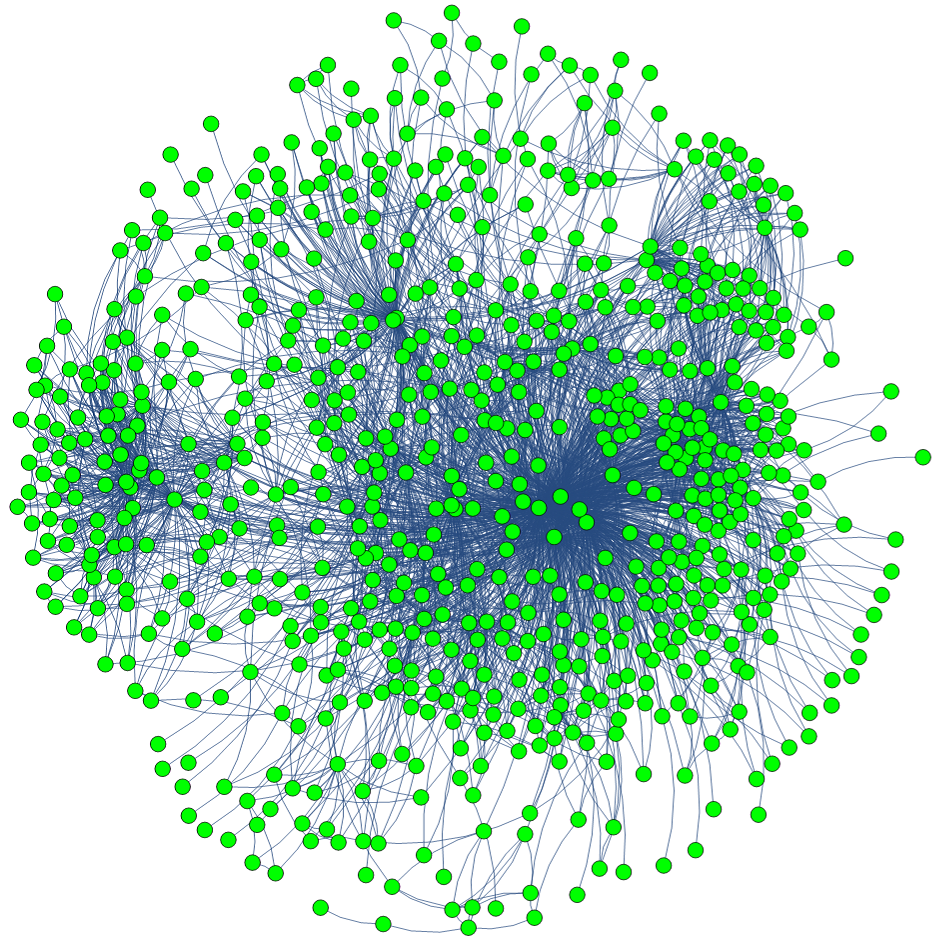
\includegraphics[width=1\linewidth]{../images/methodology-ORmodel-metabolic_centric_network.png}
		\caption{Metabolic-centric Network}
		\label{figure-metabolic-centric}
	\end{subfigure}\hfill% or \hspace{5mm} or  \hspace{0.3\textwidth}
	\begin{subfigure}{0.5\textwidth}
		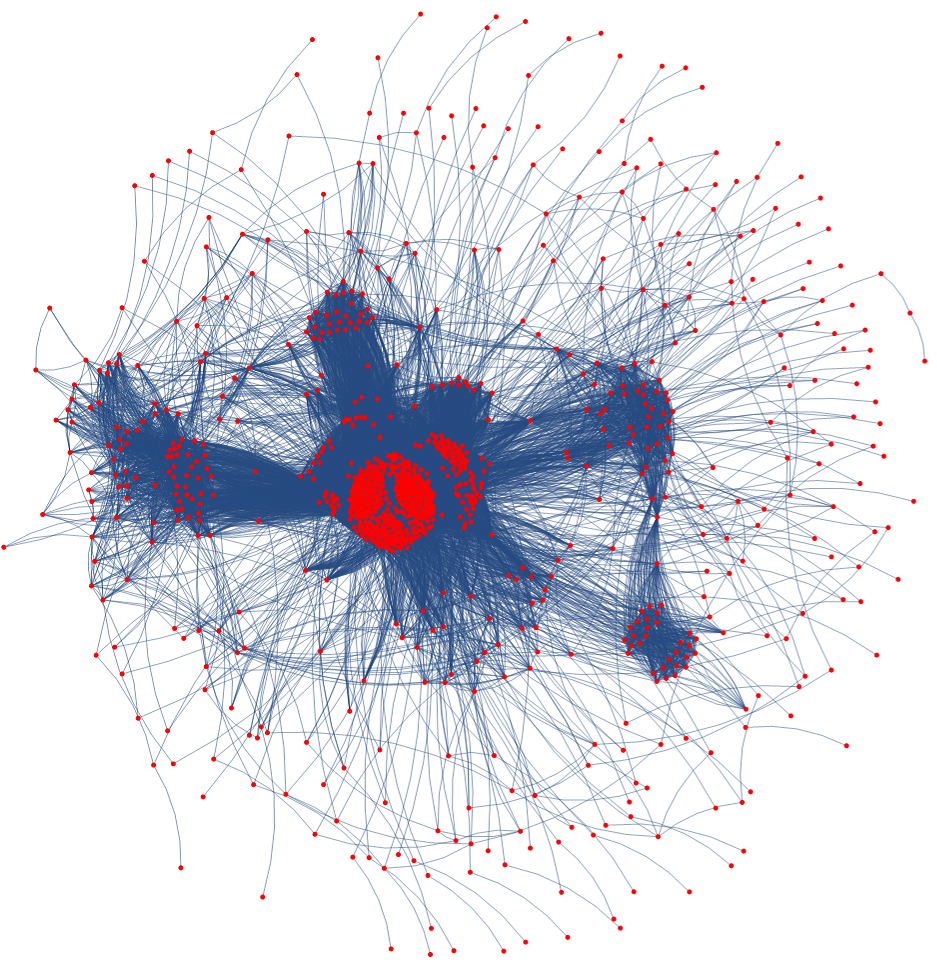
\includegraphics[width=1\linewidth]{../images/methodology-ORmodel-reaction_centric_network.png}
		\caption{Reaction-centric Network}
		\label{figure-reaction-centric}
	\end{subfigure}
	\caption{Network Representations for Homo Sapiens Metabolic Model}
	\label{figure-metabolic-networks}
\end{figure}

Studying biological metabolic systems and designed models to achieve cellular objectives like cell growth or ATP (Adenosine Triphosphate Production) necessitates various tools to be integrated with reconstructed genome-scale networks~\cite{KIM, HAO}. One of the commonly used tools is Flux Balance Analysis (FBA) as an optimization scheme. It is a constraint-based modelling approach to simulate microbial metabolisms and can be applied to biochemical-reaction networks containing the chemical transformations and flux exchanges~\cite{KAUFFMAN2003491, PRICE2004}.

While one can express the metabolic fluxes in a one-dimensional array (the so-called flux vector $V$) as
\begin{equation} %\tag{2}
	V = \begin{bmatrix}
		v_{1} \\
		v_{2} \\
		\vdots \\
		v_{r}
	\end{bmatrix}=(v_{i})\in \mathbb{R}.
	\label{solutionvector}
\end{equation}
\myequations{Fluxes Solution Vector}
$V$ contains flux exchange values for the corresponding reactions in the system and gives information about the flux distribution; hence, those can be both positive and negative real numbers. Defining a mass-balance ($S.V=0$) constraint in the FBA enables us to analyze the metabolic network operations in a steady-state solution space~\cite{KAUFFMAN2003491,PRICE2004}.
\begin{equation} %\tag{3}
	S.V = \begin{bmatrix} 
		s_{11}v_{1} + s_{12}v_{2} + \dots + s_{1r}v_{r} \\
		s_{21}v_{1} + s_{22}v_{2} + \dots + s_{2r}v_{r} \\
		\vdots \\
		s_{m1}v_{1} + s_{m2}v_{2} + \dots + s_{mr}v_{r} 
	\end{bmatrix}=
	\begin{bmatrix} 
		0 \\
		0 \\
		\vdots \\
		0
	\end{bmatrix}.
	\label{massbalanceconstraint}
\end{equation}
\myequations{Mass Balance in Steady State}
The higher amount of metabolite consideration in the set of rules, $S$, in other words, the larger matrix size by its rows amount means the more complex type of organization structure taken into account while preserving the steady-state in the whole system.

More than one steady-state solution might be present since it is impossible to identify all constraints in a cellular system~\cite{KAUFFMAN2003491}. Therefore, one can formulate an optimization approach to identify reaction network steady-states that maximize the biomass~\cite{KAUFFMAN2003491,PRICE2004} or control the production of specific metabolites~\cite{VARMA1993} within a defined objective function under the consideration of the system constraints. According to Price et al. (2004),
there are three primary purposes to generate objective functions~\cite{PRICE2004}:
\begin{itemize}
	\item[i.] to discover allowable characteristic properties in the genome-scale network reconstruction,
	\item[ii.] to mimic probable physiological functions like biomass or ATP production to be able to determine likely physiological states and
	\item[iii.] to design a genetic variant or sub-type to obtain a desired particular product.
\end{itemize}

One can express objective function coefficients in a one-dimensional array as
\begin{equation} %\tag{4}
	O =  \begin{bmatrix}
		o_{1} & o_{2} & \dots  & o_{r}\\
	\end{bmatrix}=(o_{i})\in \mathbb{R}.
	\label{objectivecoefficients}
\end{equation}
\myequations{Objective Function Coefficients Array}
As given in Eq.\eqref{biomassmaximisation}, the biomass formulation delivers the output with its non-zero coefficients, which are the decisive ones for the flux elements of $V$ to be considered.
\begin{equation} %\tag{5}
	O.V = (o_{1}v_{1} + o_{2}v_{2} + \dots + o_{r}v_{r})\in \mathbb{R}_{\ge0}.
	\label{biomassmaximisation}
\end{equation}
\myequations{Maximized Biomass}
Stoichiometric (or mass-balance) constraints were introduced so far in Eq.\eqref{stoichio} and Eq.\eqref{massbalanceconstraint}. In addition, upper and lower bounds are presented for particular fluxes in $V$ during the optimization process. The bounds are used in the reactions for uptake and secretion of any organic metabolite. In the uptake reactions, nutrients are transported to the inside of the metabolic network. In the secretion reactions, products are exported to the outside of the network. The rest of the fluxes in $V$ are used in the exchange reactions, namely the intermediate reactions in the network. The constraints influence the reactions for uptake and secretion, whereas no limitation is considered in the exchange reactions. Quantifying imported nutrients and exported outputs (resources and products) by constraining them with upper and lower bounds to fulfil a single objective function goal might significantly influence the optimization process.

 \begin{figure}[!ht]
	\begin{center}
		\makebox[\textwidth]{
			\centering
			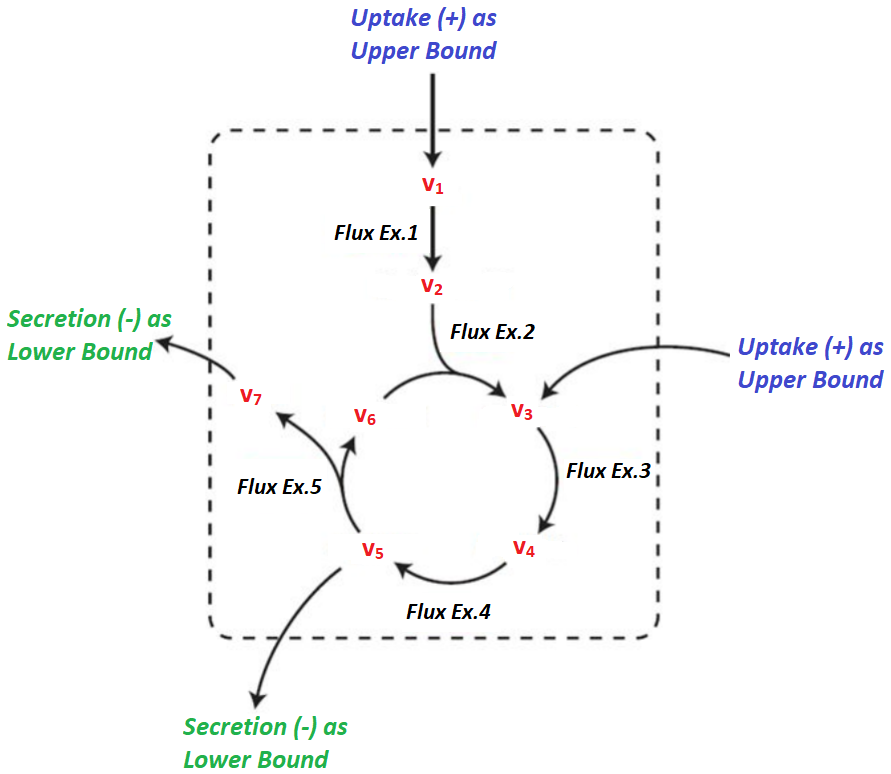
\includegraphics[width=0.57\linewidth]{../images/methodology-ORmodel-uptake_secretion_cartoon.png}}
		\caption{A Simplified Reaction-centric Network Sketch Shows The Reactions for Exchange, Uptake and Secretion.}
		\label{figure-uptake-secretion-cartoon}
	\end{center}
\end{figure}

As a summary of the above-explained series of constraints, mass-balance (Eq.\eqref{massbalanceconstraint}), upper \& lower bounds for fluxes (Fig.~\ref{figure-uptake-secretion-cartoon}), and the objective function (Eq.\eqref{objectivecoefficients}) are the three fundamental constraints that set off a linear programming problem because it is possible to formulate them linearly~\cite{PRICE2004}. The optimization result: flux vector $V$ (Eq.\eqref{solutionvector}) maximizes the objective function in the form of a flux distribution~\cite{KAUFFMAN2003491,PRICE2004}. Since each term in Eq.\eqref{biomassmaximisation} is a produced biomass expression for the fluxes, the summation of those terms will give the overall growth of the system for a single network state.

Different solution vectors of $V$ can be obtained from the linear optimization process by varying network conditions. As a compact set of rules, the stoichiometric constraints significantly influence the mass-balance equation; consequently, the solution vector $V$~\cite{Edwards2001}. A stoichiometric matrix from scratch can be formulated, ensuring the mass-balance constraints are incorporated in the reaction cycles of the investigated system. However, the homo sapiens metabolic model was taken as the set of rules in this thesis work. Varying upper \& lower flux bounds and the objective function are the two alternative approaches introduced in the following subsections to understand the model behaviour while the optimization is carried on.
\subsection*{Resource Utilization}
\addcontentsline{toc}{subsection}{Resource Utilization}%
Environmental conditions such as resource availability affect the pattern of outputs in a metabolic network. In case of fewer resources (nutrients) availability, the active production network gets more interconnected through more flux exchanges to produce the necessary input for the ongoing metabolic reactions.~\cite{PRICE2004,MAHADEVAN2003,Reed01092004,BURGARD2001}
\begin{equation} %\tag{6}
	V^{b}={v^{b}_{1}, v^{b}_{2},\dots, v^{b}_{x}}= (-a\le v^{b}_{i}\le a)\in V
	\label{constrainedfluxlist}
\end{equation}
\myequations{Constrained Fluxes List}
Let $V^{b}$ is a list of fluxes with $x$ elements randomly picked from $V$ (Eq.\eqref{solutionvector}) to be limited with the bounds: $(-a, a)$. The same tolerance in both negative and positive direction for the bounds allows the network to treat the respective flux flow as uptake or secretion based on the system need. The fluxes that are not included in $V^{b}$ are matched with extreme high boundary values so that they are not constrained while the linear optimization.
\begin{equation} %\tag{7}
	V^{e}={v^{e}_{1}, v^{e}_{2},\dots, v^{e}_{y}}= (0\le v^{e}_{i}\le 0)\in V
	\label{deletedreactions}
\end{equation}
\myequations{Deleted Fluxes List}
Assigning zero to the upper \& lower bounds suppresses the respective flux exchange in the active production network. Deleted fluxes can not be used for the uptake, secretion, nor intermediate reactions. $V^{e}$ (Eq.\eqref{deletedreactions}) is the list of fluxes with $y$ elements randomly selected from $V$ (Eq.\eqref{solutionvector}) to be discarded from the network.

Limitations on resources serve as capacity constraints defining the active reactions and reversibility of flux exchanges~\cite{Edwards2001}. Varying $x$, $y$, and $a$ to fulfil a fixed objective function, we obtain various biomass values by the linear programming algorithm.

\subsection*{Production Portfolio Diversification}
\addcontentsline{toc}{subsection}{Production Portfolio Diversification}%
The objective function can be assumed as a production plan that rules the diversity of products that metabolism takes into account to maximize cellular growth~\cite{Edwards2001}. As previously mentioned, this is because the pattern of output biomass (Eq.\eqref{biomassmaximisation}) is governed by the objective function (Eq.\eqref{objectivecoefficients}). Its non-zero coefficients force the network for an optimal solution with their value range and positive and negative signs.    

Defining a variety of sets of objective functions, each has negative or positive signs, will allow us to create a diverse group of products that the network is capable of producing. In the same direction, deleting the objective function terms up to a certain level is the second step of that diversification approach.